\documentclass[12pt,a4paper]{report}

\usepackage[T1]{fontenc}
\usepackage[utf8]{inputenc}
\usepackage[french]{babel}
\usepackage{lmodern}
\usepackage{microtype}

\usepackage{graphicx}
\usepackage{geometry}
\geometry{margin=2.5cm}

\usepackage{tikz}
\usetikzlibrary{arrows.meta, positioning, shapes.misc, shapes.geometric}

\usepackage{enumitem}
\setlist[itemize]{topsep=0.4em, itemsep=0.2em, leftmargin=1.5em}

\usepackage{fancyhdr}
\fancypagestyle{main}{
  \fancyhf{}
  \fancyhead[L]{\nouppercase{\leftmark}}
  \fancyfoot[C]{\thepage}
  \renewcommand{\headrulewidth}{0.4pt}
  \renewcommand{\footrulewidth}{0pt}
}

% Réduit les risques de lignes trop longues (overfull boxes)
\setlength{\emergencystretch}{2em}

\usepackage{booktabs}
\usepackage{longtable}
\usepackage{array}

\usepackage{xcolor}
\usepackage{hyperref}
\hypersetup{
  colorlinks=true,
  linkcolor=black,
  urlcolor=blue,
  citecolor=blue
}
\usepackage{csquotes}
\usepackage{listings}
\lstset{
  basicstyle=\ttfamily\small,
  breaklines=true,
  frame=single,
  rulecolor=\color{black!20},
  backgroundcolor=\color{black!2},
  tabsize=2
}

% ---------------------------------------------------------------------------
% Métadonnées (à adapter si besoin)
% ---------------------------------------------------------------------------
\newcommand{\rapportTitre}{Conception et réalisation d’un système d’archivage documentaire intelligent}
\newcommand{\auteurNom}{KOEVI Komi Pascal}
\newcommand{\formation}{Master Systèmes d’Information}
\newcommand{\universite}{LBS}
\newcommand{\anneeAcademique}{2025--2026}
\newcommand{\nomMinistere}{Ministère de l'Efficacité du Service Public et de Transformation Numérique (MESPTN)}
\newcommand{\directeurMemoire}{Encadrant académique : \textit{M. KONAN}}
\newcommand{\structureAccueil}{Structure d’accueil : \textit{\nomMinistere}}
\newcommand{\tuteurStage}{Référent professionnel : \textit{M. Morlé KOUDEKA}}

\title{\rapportTitre}
\author{\parbox{0.95\textwidth}{\centering
  \auteurNom\\
  \formation --- \universite\\
  \directeurMemoire\\
  \structureAccueil\\
  \tuteurStage
}}
\date{Avril 2026}

\begin{document}
% Page de garde (mise en page contrôlée, évite les débordements)
\begin{titlepage}
  \thispagestyle{empty}
  \centering
  \vspace*{2.5cm}
  {\LARGE \rapportTitre\par}
  \vspace{2.2cm}

  {\large \auteurNom\par}
  \vspace{0.3cm}
  {\formation\ --- \universite\par}
  \vspace{0.8cm}

  {\directeurMemoire\par}
  {\structureAccueil\par}
  {\tuteurStage\par}

  \vfill
  {Avril 2026\par}
\end{titlepage}

% Préliminaires (numérotation romaine)
\pagenumbering{roman}
\setcounter{page}{1}

\listoffigures
% \listoftables % à activer si des tableaux sont ajoutés

\clearpage
\tableofcontents
\clearpage

\chapter*{Résumé}
\addcontentsline{toc}{chapter}{Résumé}
Un document scanné n’est pas encore une archive. Dans les administrations publiques, la gestion documentaire repose encore largement sur des supports papier et sur des pratiques de classement hétérogènes, rendant l’accès à l’information difficile, lent et peu fiable. Au \nomMinistere{}, des milliers de documents anciens, datant de plus de dix ans, devaient être numérisés dans un délai contraint, tout en restant exploitables au quotidien.

L’enjeu principal consistait ainsi à transformer un volume important de documents numérisés en archives structurées, correctement nommées, classées et facilement retrouvables.

Ce rapport présente la conception et la réalisation d’un système d’archivage numérique déployé en environnement \textit{on-premise}. La solution proposée permet l’ingestion automatique des documents depuis plusieurs scanners via des dossiers partagés, puis déclenche une chaîne de traitement basée sur des techniques d’intelligence artificielle : reconnaissance optique de caractères (OCR), extraction d’informations, structuration des données et génération de métadonnées. Ces traitements permettent de proposer automatiquement un renommage et un classement conformes aux règles définies par le ministère, tout en laissant à l’utilisateur la possibilité de valider ou corriger les résultats via une interface web dédiée.

L’architecture du système repose sur une approche microservices, garantissant la scalabilité, la résilience et la modularité de la solution. En complément, un assistant conversationnel permet d’interroger le contenu documentaire en langage naturel. Les réponses sont générées à partir d’un contexte extrait des documents archivés, selon une approche de recherche sémantique couplée à la génération augmentée par récupération (\textit{RAG}), améliorant significativement l’accès à l’information.

Ainsi, la solution mise en place permet d’industrialiser le processus d’archivage numérique en réduisant les tâches manuelles, en améliorant la qualité et la cohérence du classement, et en garantissant la traçabilité des opérations. Elle répond également aux exigences de sécurité et de souveraineté grâce à un déploiement en environnement interne.

\chapter*{Liste des acronymes}
\addcontentsline{toc}{chapter}{Liste des acronymes}
\begin{description}[leftmargin=2.5cm, style=nextline]
  \item[API] \textit{Application Programming Interface}
  \item[GED] Gestion Électronique des Documents
  \item[IA] Intelligence Artificielle
  \item[IAM] \textit{Identity and Access Management}
  \item[LLM] \textit{Large Language Model}
  \item[MFA] \textit{Multi-Factor Authentication}
  \item[OCR] \textit{Optical Character Recognition}
  \item[RBAC] \textit{Role-Based Access Control}
  \item[RAG] \textit{Retrieval-Augmented Generation}
  \item[RAGAS] \textit{Retrieval-Augmented Generation Assessment}
  \item[SSO] \textit{Single Sign-On}
  \item[TLS] \textit{Transport Layer Security}
\end{description}

% Corps du document (numérotation arabe + en-têtes/pieds de page)
\pagenumbering{arabic}
\pagestyle{main}

\chapter*{Introduction}
\addcontentsline{toc}{chapter}{Introduction}
Dans les administrations publiques, la gestion documentaire repose encore largement sur des supports papier et sur des pratiques de classement souvent hétérogènes. Cette situation complique l’accès à l’information, accroît les risques de perte ou de dégradation des documents, et limite l’efficacité opérationnelle des services.

Dans ce contexte, le \nomMinistere{} est confronté à un enjeu majeur : numériser et archiver un volume important de documents anciens, datant de plus de dix ans, dans un délai contraint, en garantissant leur exploitation à long terme. Toutefois, la simple numérisation ne constitue pas une solution suffisante. Un document scanné mais mal nommé, mal classé ou difficilement retrouvable perd rapidement sa valeur informationnelle. À grande échelle, les opérations manuelles de tri, de renommage et de recherche deviennent coûteuses, sources d’erreurs et difficilement maintenables.

Dès lors, la problématique suivante se pose : comment concevoir une chaîne d’archivage numérique capable de traiter efficacement un volume important de documents numérisés, en réduisant les interventions manuelles, en améliorant la qualité du classement, en garantissant la traçabilité des opérations et en permettant une recherche rapide et fiable, dans un environnement sécurisé et déployé en local (\textit{on-premise}) ?

Pour répondre à cette problématique, le projet \textbf{Document Archiving System (DAS)} vise à concevoir et à mettre en œuvre une solution d’archivage numérique automatisée. Cette solution permet notamment l’ingestion automatique des documents depuis les scanners, l’extraction d’informations via des techniques d’OCR, ainsi que l’assistance au classement et au renommage selon des règles définies. Elle propose également une interface web facilitant la consultation, la recherche et la validation des documents. Par ailleurs, des mécanismes de suivi et de traçabilité sont intégrés afin d’assurer une exploitation fiable dans la durée, tout en respectant les exigences de souveraineté et de sécurité propres à un déploiement interne.

En complément, la solution intègre un assistant conversationnel permettant d’interroger le contenu documentaire et d’obtenir des réponses contextualisées, en s’appuyant sur une approche de recherche sémantique couplée à des techniques de génération augmentée par récupération (\textit{RAG}).

Ce rapport est structuré en trois parties. La première présente le cadre de la mission (structure d’accueil, contexte, existant et analyse des besoins). La deuxième détaille la conception et la réalisation de la solution (architecture, modèle de données, implémentation et déploiement). La troisième aborde les aspects d’exploitation, de sécurité et d’évaluation.

\part{Cadre de la mission et expression des besoins}
\chapter{Présentation de la structure d’accueil}
Ce chapitre présente la structure d’accueil de la mission, le \nomMinistere{}, ainsi que le contexte dans lequel s’inscrit le projet. Il décrit les missions du ministère, son organisation générale, le rôle du service d’accueil dans la gestion documentaire, et les responsabilités confiées dans le cadre de la mission.

\section{Missions et organisation}
Le \nomMinistere{} est une administration publique dont la mission principale est d’améliorer la qualité et l’efficacité des services rendus aux usagers, tout en accompagnant la transformation numérique des processus administratifs internes.

Dans ce cadre, la production, la circulation et la conservation des documents administratifs (courriers, notes, arrêtés, pièces justificatives, dossiers ou comptes rendus) occupent une place centrale dans le fonctionnement quotidien des services.

La mission s’est déroulée au sein d’une équipe en charge des outils numériques et de la gestion documentaire. Cette équipe intervient notamment sur :
\begin{itemize}
  \item la mise à disposition d’outils dédiés à la numérisation et à l’archivage des documents ;
  \item la structuration de l’information (classement, métadonnées, organisation documentaire) ;
  \item l’accompagnement des utilisateurs, en particulier les secrétariats et les services métier ;
  \item la sécurisation et la conformité des solutions déployées dans l’environnement interne.
\end{itemize}

\section{Contexte de la mission}
La mission s’inscrit dans un projet de numérisation et d’archivage massif de documents anciens, datant de plus de dix ans, avec un double objectif :
\begin{itemize}
  \item absorber un volume important de documents dans un délai contraint ;
  \item mettre en place un dispositif pérenne, exploitable au quotidien par les utilisateurs.
\end{itemize}

Compte tenu de la sensibilité des informations traitées et des exigences de souveraineté, la solution doit être déployée en environnement local (\textit{on-premise}). Elle doit également s’intégrer aux pratiques existantes des services, caractérisées par :
\begin{itemize}
  \item l’utilisation de plusieurs scanners ;
  \item le recours à des dossiers partagés sur le réseau interne ;
  \item la nécessité d’un fonctionnement basé sur un principe de validation humaine (\og proposer puis valider \fg{}) afin de garantir la fiabilité du classement.
\end{itemize}

\section{Rôle et responsabilités}
En tant que développeur fullstack, j’ai été chargé de la conception et de la mise en œuvre de la solution, en collaboration avec l’équipe technique et les utilisateurs finaux.

Les principales responsabilités ont porté sur :
\begin{itemize}
  \item la conception de l’architecture applicative et du pipeline de traitement (ingestion, OCR, extraction, indexation) ;
  \item le développement des services backend (API, orchestration asynchrone) ainsi que des interfaces web dédiées à la validation et à la consultation ;
  \item la mise en place du déploiement en environnement \textit{on-premise} (Docker Compose) et des premiers éléments d’exploitabilité (journalisation, métriques, tableaux de bord) ;
  \item l’intégration des contraintes métier, notamment les règles de nommage et de classement, en tenant compte des retours utilisateurs.
\end{itemize}

\chapter{État de l’existant et problématique terrain}
\section{Processus d’archivage avant projet}
Avant le projet, l’archivage reposait majoritairement sur un enchaînement d’actions manuelles : réception d’un document papier, scan, renommage du fichier, classement dans une arborescence partagée, puis transmission au service concerné. La recherche d’un document s’effectuait principalement par navigation dans des dossiers et par mémoire des utilisateurs.

Ce fonctionnement, acceptable à faible volume, montre rapidement ses limites lorsque le nombre de documents augmente :
\begin{itemize}
  \item incohérences de nommage (fichiers difficiles à identifier) ;
  \item classement variable selon les personnes et les services ;
  \item doublons et pertes de documents lors des transferts ;
  \item absence de traçabilité complète des actions (qui a classé, modifié, validé) ;
  \item recherche lente, surtout lorsque le contenu du document n’est pas indexé.
\end{itemize}

\section{Contraintes et enjeux}
Le contexte ministériel impose plusieurs contraintes fortes :
\begin{itemize}
  \item \textbf{Volumétrie} : plusieurs milliers de documents à traiter, avec des pics de charge ;
  \item \textbf{Hétérogénéité} : formats et qualités de scan variables (PDF, images, documents bruités) ;
  \item \textbf{Confidentialité} : documents potentiellement sensibles (données personnelles, décisions, actes) ;
  \item \textbf{Délais} : nécessité d’un traitement rapide et industrialisé ;
  \item \textbf{Disponibilité des utilisateurs} : les secrétariats doivent pouvoir utiliser l’outil sans complexité technique.
\end{itemize}

Les enjeux associés sont : garantir un archivage \textbf{fiable} et \textbf{traçable}, améliorer l’accès à l’information (recherche par contenu) et réduire durablement la charge manuelle (tri/renommage/classement), tout en respectant un déploiement \textit{on-premise}.

\chapter{Besoins et cahier des charges}
Ce chapitre présente les besoins identifiés pour la mise en place du système, ainsi que les critères permettant d’évaluer l’adéquation de la solution proposée. Il distingue les besoins fonctionnels, les exigences non fonctionnelles et les critères d’acceptation.

\section{Besoins fonctionnels}
Les besoins fonctionnels définissent les fonctionnalités attendues du système. Ils ont été identifiés en collaboration avec les utilisateurs métiers et l’équipe technique.
\begin{itemize}
  \item \textbf{Ingestion multi-scanners} : récupération automatique des documents numérisés via des dossiers partagés réseau et/ou via une API d’upload.
  \item \textbf{Reconnaissance optique de caractères (OCR)} : extraction du texte à partir des documents scannés afin de rendre leur contenu exploitable.
  \item \textbf{Extraction et structuration des données} : identification des informations pertinentes (objet, expéditeur/destinataire, numéros, dates, type de document).
  \item \textbf{Renommage et classement assistés} : proposition automatique d’un nom de fichier et d’un emplacement de classement conformes aux règles définies par le ministère.
  \item \textbf{Validation utilisateur} : possibilité pour les secrétariats de valider, modifier ou corriger les propositions avant archivage définitif.
  \item \textbf{Recherche documentaire} : recherche plein texte et recherche sémantique permettant de retrouver rapidement un document à partir de son contenu.
  \item \textbf{Gestion documentaire (GED)} : gestion d’une arborescence de dossiers et fichiers, avec fonctionnalités de consultation, téléchargement et éventuellement gestion de versions.
  \item \textbf{Audit et traçabilité} : journalisation des actions et des changements d’état (création, validation, modification, déplacement, suppression).
\end{itemize}

\section{Besoins non fonctionnels}
Les besoins non fonctionnels décrivent les contraintes techniques et qualitatives auxquelles le système doit répondre.
\begin{itemize}
  \item \textbf{Sécurité} : déploiement en environnement \textit{on-premise}, limitation de la surface d’exposition, contrôle des accès et traçabilité des actions.
  \item \textbf{Performance} : capacité à absorber des volumes importants de documents et à traiter les flux de manière asynchrone.
  \item \textbf{Disponibilité} : continuité de service malgré l’indisponibilité temporaire de certains composants, grâce à une architecture basée sur des messages.
  \item \textbf{Maintenabilité} : architecture modulaire reposant sur des composants découplés, facilitant les évolutions et la maintenance.
  \item \textbf{Exploitabilité} : mise en place de mécanismes de supervision incluant logs centralisés, métriques, alertes et tableaux de bord opérationnels.
\end{itemize}

\section{Critères d’acceptation}
Afin de valider la conformité de la solution aux besoins exprimés, plusieurs critères d’acceptation ont été définis :
\begin{itemize}
  \item \textbf{Automatisation du flux} : tout document déposé via un scanner ou une API est pris en charge automatiquement, sans intervention technique.
  \item \textbf{Délai de traitement} : un document standard est traité (de l’ingestion à la proposition de validation) dans un délai compatible avec l’usage opérationnel (objectif indicatif : quelques minutes).
  \item \textbf{Qualité des propositions} : les suggestions de classification et de renommage sont suffisamment pertinentes pour réduire significativement les corrections manuelles.
  \item \textbf{Efficacité de la recherche} : il est possible de retrouver rapidement un document à partir de mots-clés ou de son contenu.
  \item \textbf{Traçabilité des actions} : les opérations critiques (création, validation, modification, déplacement, suppression) sont systématiquement journalisées.
  \item \textbf{Exploitabilité technique} : l’équipe dispose d’indicateurs fiables (état du pipeline, erreurs, latences) ainsi que de mécanismes de supervision et de reprise en cas d’incident.
\end{itemize}

\chapter{Méthodologie et organisation du projet}
\section{Démarche}
Ce chapitre présente la démarche méthodologique adoptée pour la conduite du projet, ainsi que son organisation, depuis le cadrage initial jusqu’à la mise en production progressive de la solution.

Une approche itérative et incrémentale, inspirée des méthodes agiles (Scrum), a été retenue afin de livrer rapidement une première version fonctionnelle du système, puis d’enrichir progressivement ses fonctionnalités en fonction des retours des utilisateurs.

Cette démarche a permis de réduire les risques, d’améliorer l’adéquation aux besoins métiers et de favoriser une validation continue des choix techniques.

Les principales étapes ont été les suivantes :
\begin{itemize}
  \item \textbf{Cadrage fonctionnel} : recueil des besoins auprès des parties prenantes (secrétariats, équipe technique), identification des contraintes métier et définition des cas d’usage prioritaires ;
  \item \textbf{Prototypage initial} : mise en place d’un premier pipeline minimal (ingestion $\rightarrow$ OCR $\rightarrow$ stockage) afin de valider les choix techniques ;
  \item \textbf{Itérations successives} : ajout progressif des modules d’extraction, d’assistance intelligente (classification, renommage) et de recherche documentaire ;
  \item \textbf{Intégration des interfaces utilisateur} : développement des interfaces de consultation et de validation, avec prise en compte des retours terrain ;
  \item \textbf{Stabilisation et mise en production} : amélioration de la robustesse, mise en place de l’observabilité (logs, métriques, alertes) et préparation au déploiement en environnement \textit{on-premise}.
\end{itemize}

L’implication des parties prenantes a été un élément clé de la démarche. Des échanges réguliers avec les utilisateurs finaux ont permis d’ajuster les fonctionnalités, notamment sur les règles de classement et les interfaces de validation.

Les principaux risques identifiés concernaient :
\begin{itemize}
  \item la qualité et la variabilité des documents scannés (impact sur l’OCR) ;
  \item l’hétérogénéité des formats documentaires ;
  \item la nécessité de garantir un contrôle humain sur les décisions automatisées.
\end{itemize}

Ces risques ont été atténués par :
\begin{itemize}
  \item une architecture asynchrone basée sur un système de messagerie (RabbitMQ), permettant de fiabiliser le traitement ;
  \item la mise en place d’un workflow de validation utilisateur (\og proposer puis valider \fg{}) ;
  \item une approche progressive permettant d’ajuster les traitements en fonction des résultats observés.
\end{itemize}

\section{Organisation et planification}
Le projet a été structuré selon une logique d’itérations courtes (\textit{sprints}), avec des livraisons incrémentales permettant de valider rapidement les fonctionnalités développées.

Les principaux livrables ont été organisés comme suit :
\begin{itemize}
  \item (i) ingestion automatique des documents ;
  \item (ii) OCR et stockage ;
  \item (iii) extraction des informations et gestion des métadonnées ;
  \item (iv) assistance au classement et au renommage ;
  \item (v) interface utilisateur et moteur de recherche ;
  \item (vi) observabilité, supervision et durcissement du système.
\end{itemize}

Chaque itération donnait lieu à une démonstration auprès des utilisateurs et de l’équipe technique, permettant de recueillir des retours et d’ajuster les développements suivants. Cette boucle de feedback a contribué à améliorer progressivement la pertinence fonctionnelle et l’ergonomie du système.

\part{Conception et réalisation de la solution}

\chapter{Vue d’ensemble du système}
\section{Architecture générale}
Le système proposé repose sur une architecture orientée \textbf{microservices}, développée principalement avec \textbf{Python/FastAPI} pour le backend et \textbf{Next.js} pour le frontend. Ce choix permet de structurer l’application en composants indépendants, chacun responsable d’une fonctionnalité spécifique.

Les échanges entre les services de traitement sont assurés de manière \textbf{asynchrone} à l’aide de \textbf{RabbitMQ}. Cette approche améliore la résilience globale du système et facilite la gestion de la charge, notamment pour des opérations intensives comme l’OCR et l’extraction d’informations.

Enfin, cette architecture favorise la \textbf{scalabilité}, en permettant de dimensionner indépendamment les services les plus sollicités.

\begin{figure}[h!]
\centering
\resizebox{0.98\textwidth}{!}{%
\begin{tikzpicture}[
  font=\small,
  x=1cm, y=1cm,
  service/.style={rounded corners=2pt, draw=black!45, fill=blue!8, align=center, text width=3.2cm, inner xsep=7pt, inner ysep=6pt},
  bus/.style={rounded corners=2pt, draw=black!45, fill=orange!12, align=center, text width=3.2cm, inner xsep=7pt, inner ysep=6pt},
  serviceSmall/.style={rounded corners=2pt, draw=black!45, fill=blue!8, align=center, text width=2.8cm, inner xsep=7pt, inner ysep=6pt},
  infra/.style={rounded corners=2pt, draw=black!45, fill=green!10, align=center, text width=4.0cm, inner xsep=7pt, inner ysep=6pt},
  obs/.style={rounded corners=2pt, draw=black!45, fill=gray!10, align=center, text width=4.8cm, inner xsep=7pt, inner ysep=6pt},
  main/.style={-Latex, draw=black!70, line width=0.9pt},
  aux/.style={-Latex, draw=black!45, line width=0.55pt},
  dottedline/.style={-Latex, draw=black!40, line width=0.55pt, dashed}
]
% Rangée 1 (ingestion) — plus d’espace vertical
\node[service] (scan)   at (0, 3.6) {Scanners\\(dossiers partagés)};
\node[service] (listen) at (4, 3.6) {Scan Listener\\(optionnel)};
\node[service] (upload) at (8, 3.6) {Upload Service\\\texttt{POST /upload}};
\node[bus]     (mq)     at (12,3.6) {RabbitMQ\\(événements)};

% Rangée 2 (traitement + accès)
\node[service] (ocr)     at (0, 1.4) {OCR Service\\(Tesseract)};
\node[service] (extract) at (4, 1.4) {Extraction Service\\(Docling + chunking\\+ embeddings)};
\node[service] (llm)     at (8, 1.4) {LLM Service\\(classification\\\& renommage)};
\node[service] (route)   at (12,1.4) {Routing Service\\(API / UI)};
\node[serviceSmall] (minioMgr) at (12,0.1) {MinIO Manager};

% Infrastructure (en dessous) — plus d’espace vertical
\node[infra] (minio) at (6, -1.3) {MinIO\\(stockage objets)};
\node[infra] (pg)    at (2, -1.3) {PostgreSQL + pgvector\\(métadonnées, RBAC,\\index vectoriel)};
\node[infra] (redis) at (12,-1.3) {Redis\\(cache/état)};
\node[obs]   (obs)   at (6, -3.3) {Observabilité\\Prometheus • Grafana\\Loki • Vector};

% Flèche d’évolution (process) — simple, gauche→droite, puis seconde rangée
\draw[main] (scan) -- (listen);
\draw[main] (listen) -- (upload);
\draw[main] (upload) -- (mq);
\draw[main] (mq.south) -- (ocr.north);
\draw[main] (ocr) -- (extract);
\draw[main] (extract) -- (llm);
\draw[main] (llm) -- (route);

% Liens secondaires (courts, sans croisement)
\draw[aux] (upload.south) -- ++(0,-0.45) -| (minio.north);
\draw[aux] (ocr.south) -- ++(0,-0.45) -| (minio.north);
\draw[aux] (extract.south) -- (pg.north);
\draw[aux] (extract.south) -- ++(0,-0.45) -| (minio.north);
\draw[aux] (route.south) -- (redis.north);
\draw[aux] (minioMgr.west) -- ++(-0.5,0) |- (minio.east);

% Observabilité (pointillé) — quelques liens seulement
\draw[dottedline] (obs.north) -- (minio.south);
\draw[dottedline] (obs.north west) -- ++(-1.0,1.0) |- (upload.south);
\draw[dottedline] (obs.north east) -- ++(1.0,1.0) |- (route.south);
\end{tikzpicture}%
}
\vspace{0.2em}
\footnotesize \textbf{Légende :} bleu = microservices,\; vert = infrastructure,\; pointillé = supervision.


\caption{Architecture générale de la solution d’archivage documentaire intelligente (\textit{on-premise}).}
\label{fig:archi-generale}
\end{figure}

\subsection{Microservices métier}
Le système est composé de plusieurs microservices spécialisés :
\begin{itemize}
  \item \textbf{Upload Service} : assure la réception des documents, leur stockage initial dans MinIO et la publication d’un message dans le système de messagerie pour déclencher le traitement.
  \item \textbf{OCR Service} : réalise la reconnaissance de texte à partir des documents numérisés en s’appuyant sur Tesseract.
  \item \textbf{Extraction Service} : extrait les informations pertinentes, effectue un découpage en segments (\textit{chunking}), génère des \textit{embeddings} et indexe les données dans PostgreSQL via l’extension pgvector.
  \item \textbf{Routing Service} : constitue l’API principale exposée au frontend. Il permet la consultation, la recherche de documents et l’intégration d’une recherche avancée basée sur le paradigme RAG (\textit{Retrieval-Augmented Generation}).
  \item \textbf{Language Model Service} : gère les interactions avec un \textbf{modèle de langage local}, notamment pour la classification automatique, le renommage intelligent et les fonctionnalités de chat.
  \item \textbf{Scan Listener Service} : surveille un dossier de dépôt de scans et déclenche automatiquement leur envoi vers le service d’upload.
  \item \textbf{MinIO Manager} : fournit des opérations de gestion des fichiers (déplacement, suppression, génération de liens sécurisés, organisation et fusion de documents PDF).
\end{itemize}

\subsection{Infrastructure}
L’infrastructure du système repose sur plusieurs composants clés :
\begin{itemize}
  \item \textbf{PostgreSQL} (avec pgvector) : utilisé pour le stockage des métadonnées, la gestion des droits d’accès (RBAC), l’organisation des documents ainsi que l’indexation vectorielle.
  \item \textbf{MinIO} : assure le stockage objet des fichiers numérisés.
  \item \textbf{RabbitMQ} : joue le rôle de bus de messages pour orchestrer les différentes étapes du pipeline de traitement.
  \item \textbf{Redis} : utilisé comme composant applicatif pour la gestion du cache et de certains états côté application.
  \item \textbf{Outils d’observabilité} (Prometheus, Grafana, Loki, Vector) : permettent de superviser le système, collecter des métriques et analyser les logs.
\end{itemize}

\section{Flux de traitement d’un document}
Le traitement d’un document suit une chaîne bien définie. Dans un premier temps, les documents numérisés sont déposés dans un dossier surveillé ou envoyés directement via l’API d’upload. Le \textbf{Scan Listener Service} (optionnel) détecte automatiquement les nouveaux fichiers et les transmet au \textbf{Upload Service}.

Une fois le document reçu, celui-ci est stocké dans \textbf{MinIO} et un message est publié dans \textbf{RabbitMQ} pour signaler l’arrivée d’un nouveau document. Le \textbf{OCR Service} consomme ce message, effectue la reconnaissance de texte, puis publie un nouvel événement indiquant la fin de cette étape.

Le \textbf{Extraction Service} prend ensuite le relais pour analyser le contenu du document, extraire les informations pertinentes, générer des \textit{embeddings} et indexer les données dans \textbf{PostgreSQL}. Parallèlement, les fichiers sont organisés et conservés dans MinIO. Le flux nominal peut être résumé comme suit :

\begin{figure}[h!]
\centering
\resizebox{0.98\textwidth}{!}{%
\begin{tikzpicture}[
  font=\small,
  node distance=8mm and 12mm,
  proc/.style={rounded corners=2pt, draw=black!40, fill=blue!8, align=center, inner xsep=8pt, inner ysep=7pt, minimum height=9mm},
  store/.style={rounded corners=2pt, draw=black!40, fill=green!10, align=center, inner xsep=8pt, inner ysep=7pt, minimum height=9mm},
  line/.style={-Latex, draw=black!60, line width=0.6pt}
]
\node[proc] (s1) {Scan\\(dossier partagé)};
\node[proc, right=of s1] (s2) {Upload Service\\\texttt{/upload}};
\node[proc, right=of s2] (s3) {RabbitMQ\\\footnotesize document.uploaded};
\node[proc, right=of s3] (s4) {OCR Service\\(Tesseract)};
\node[proc, right=of s4] (s5) {RabbitMQ\\\footnotesize ocr.completed};
\node[proc, right=of s5] (s6) {Extraction Service\\(chunking +\\ embeddings)};
\node[proc, right=of s6] (s7) {LLM\\(classification\\& renommage)};
\node[proc, below=10mm of s6] (s8) {Routing + Frontend\\(recherche/validation)};

\node[store, below=10mm of s2] (minio) {MinIO\\(fichiers)};
\node[store, below=10mm of s6] (pg) {PostgreSQL + pgvector\\(métadonnées + index)};

\draw[line] (s1) -- (s2);
\draw[line] (s2) -- (s3);
\draw[line] (s3) -- (s4);
\draw[line] (s4) -- (s5);
\draw[line] (s5) -- (s6);
\draw[line] (s6) -- (s7);

\draw[line] (s2) -- (minio);
\draw[line] (s4) -- (minio);
\draw[line] (s6) -- (minio);
\draw[line] (s6) -- (pg);
\draw[line] (s7) |- (pg);
\draw[line] (pg) |- (s8);
\draw[line] (minio) |- (s8);
\end{tikzpicture}
}


\caption{Flux de traitement d’un document, de l’ingestion à la recherche et à la validation.}
\label{fig:flux-traitement}
\end{figure}

\begin{figure}[h!]
\centering
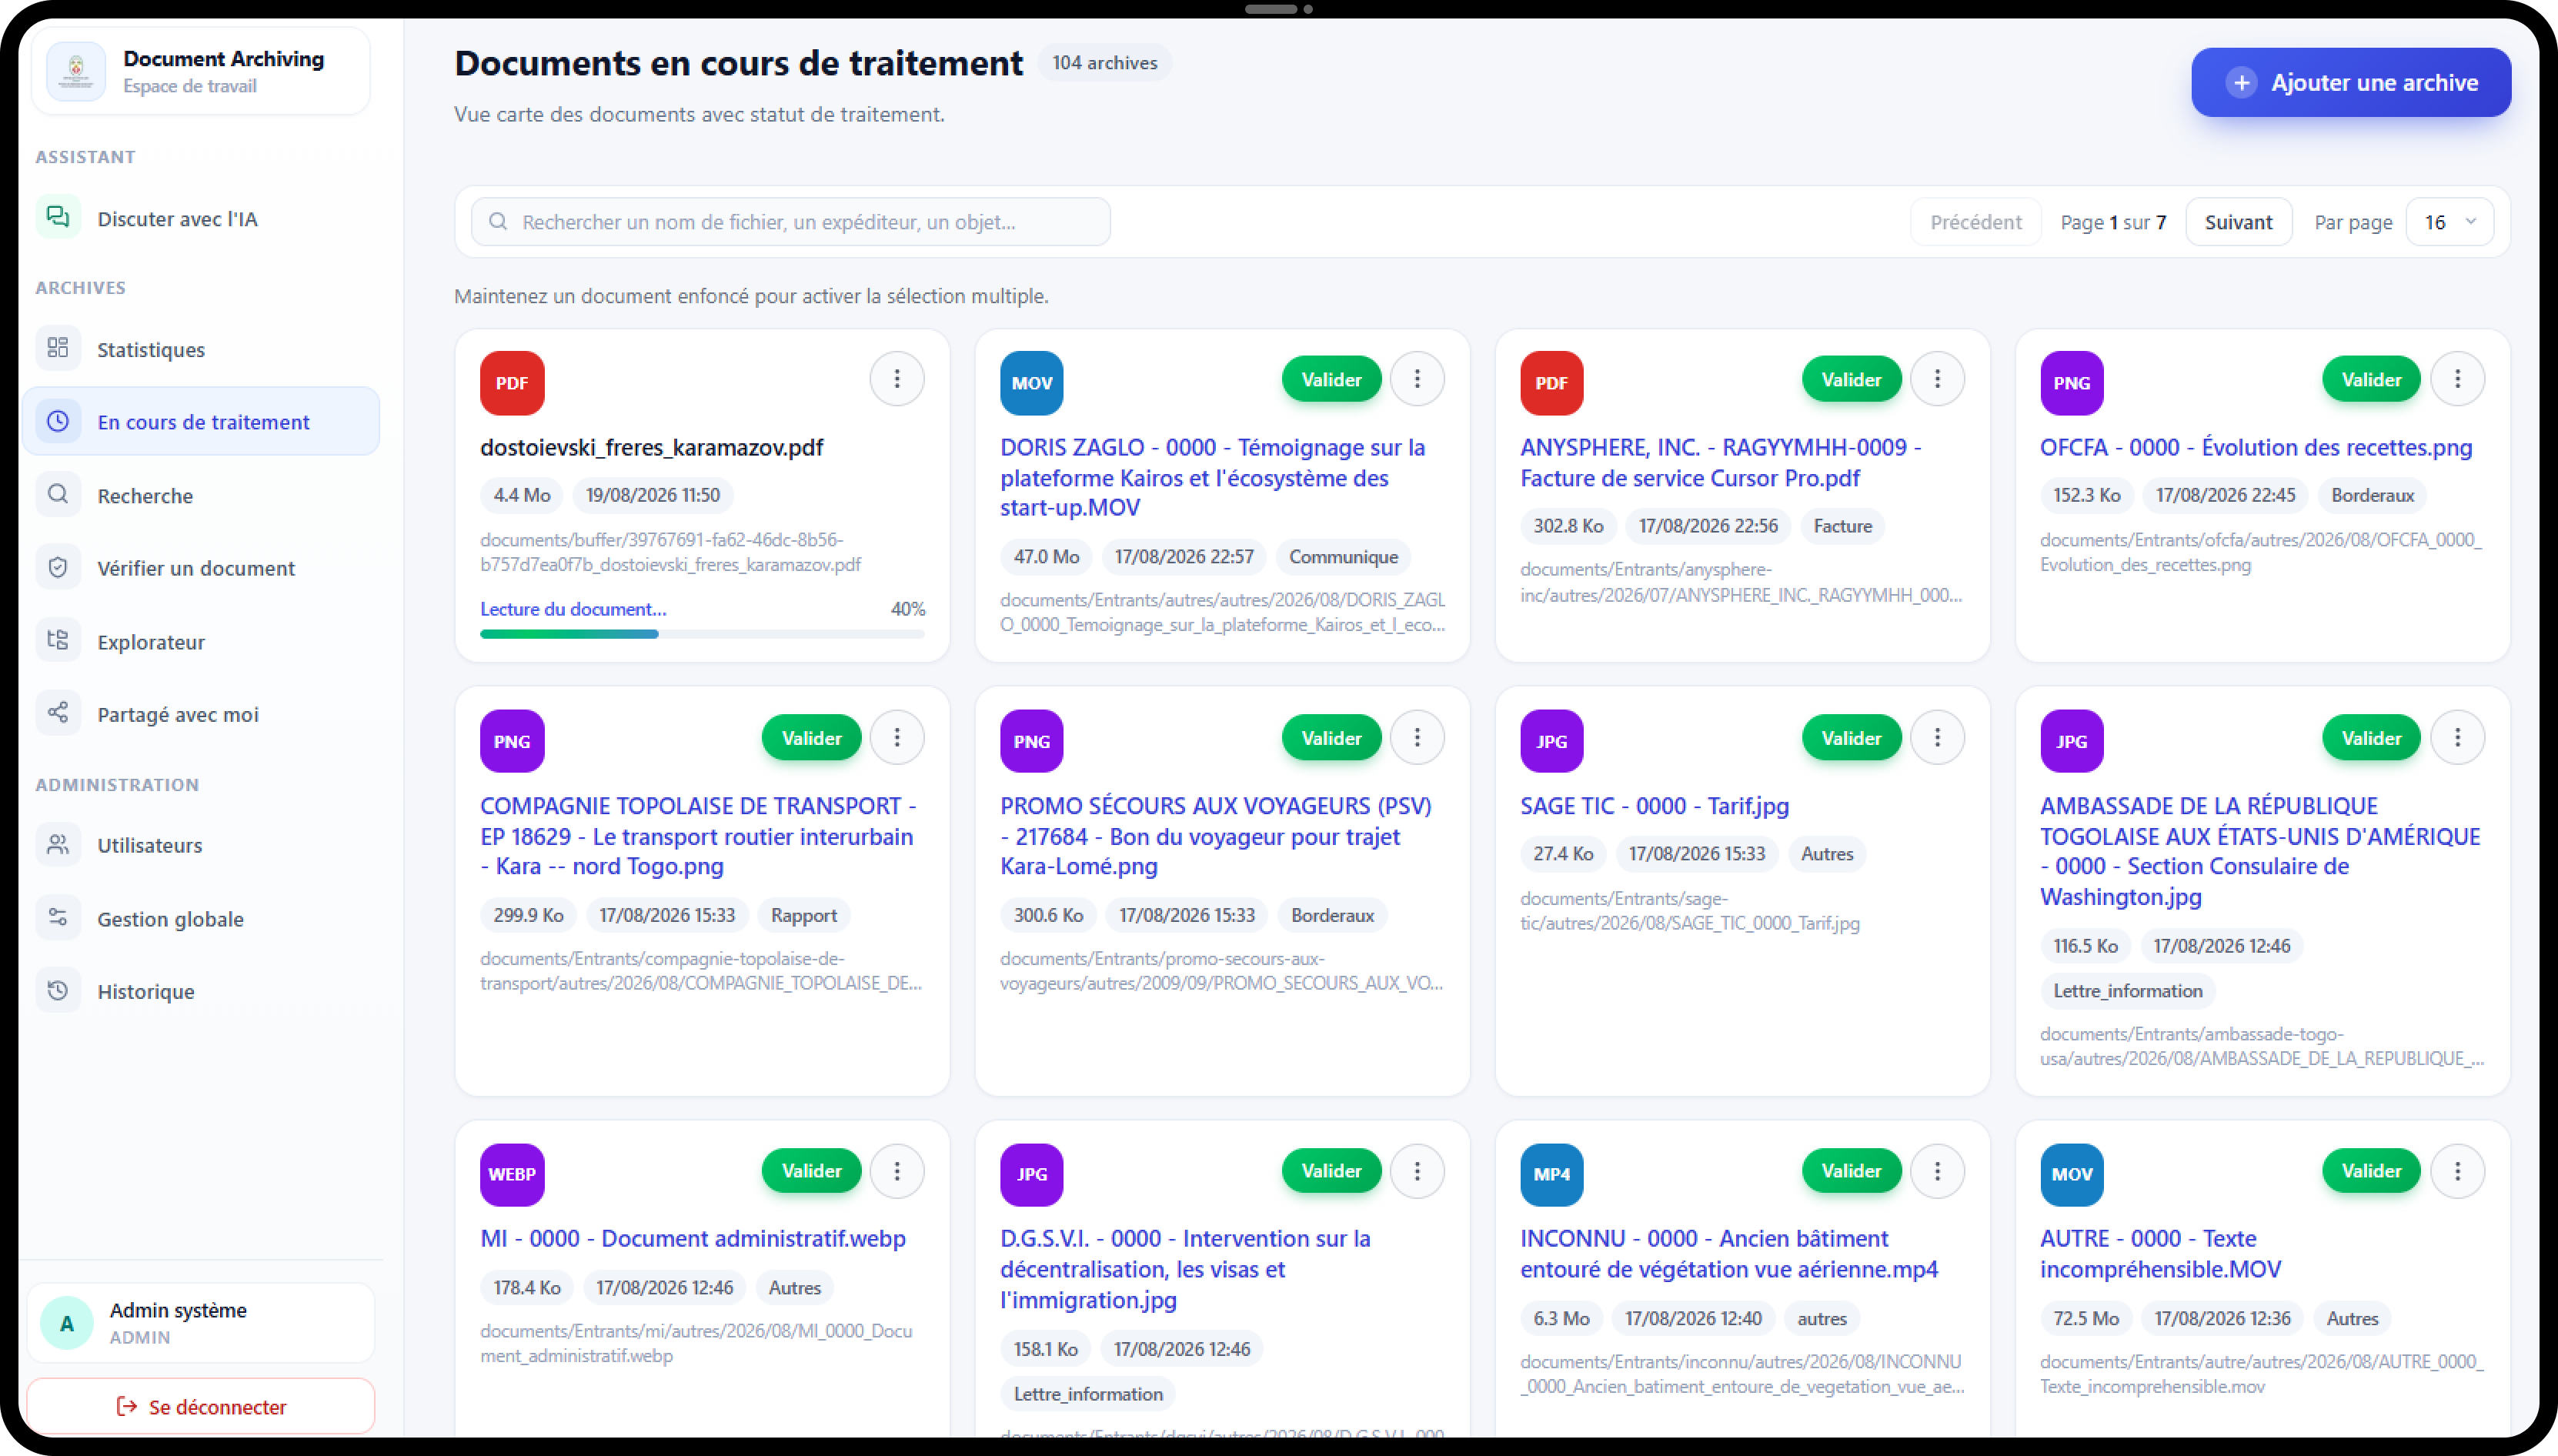
\includegraphics[width=0.98\textwidth]{images/screens/Traitement_documents.png}
\caption{Interface de suivi des documents en cours de traitement et de validation.}
\label{fig:ui-traitement-docs}
\end{figure}

Enfin, le \textbf{Routing Service}, couplé au frontend \textbf{Next.js}, permet aux utilisateurs d’accéder aux documents, d’effectuer des recherches avancées et de valider les opérations réalisées.

\section{Justification du choix microservices}
Les principaux avantages observés dans ce projet :
\begin{itemize}
  \item \textbf{Scalabilité ciblée} : les services lourds (OCR/extraction) peuvent être répliqués indépendamment.
  \item \textbf{Résilience} : le traitement est asynchrone ; une indisponibilité temporaire d’un service n’interrompt pas l’ingestion.
  \item \textbf{Séparation des responsabilités} : ingestion, OCR, extraction, API, IA et stockage sont découplés.
  \item \textbf{Évolutivité} : ajout futur de nouveaux traitements (signature, versioning avancé, nouveaux modèles IA).
\end{itemize}

\chapter{Modèle de données et stockage}
Ce chapitre décrit les choix réalisés en matière de stockage des données et de structuration des informations. Il présente l’organisation du stockage des fichiers, le modèle relationnel utilisé pour les métadonnées, ainsi que le mécanisme d’indexation sémantique permettant la recherche avancée.

\section{Stockage des fichiers (MinIO)}
Les fichiers sont stockés dans un système de stockage objet basé sur MinIO, au sein d’un bucket dédié (\texttt{documents}). Ce choix permet de garantir une gestion efficace des fichiers volumineux, tout en assurant une bonne scalabilité et une compatibilité avec les standards S3.

Lors de l’ingestion, les documents sont initialement stockés dans un préfixe tampon (par exemple \texttt{buffer/}). Ce stockage intermédiaire permet de séparer les fichiers en cours de traitement des documents validés. Une fois les traitements effectués (OCR, extraction, classification), les fichiers peuvent être déplacés et renommés afin de refléter leur organisation logique dans l’arborescence documentaire.

Par ailleurs, des URLs pré-signées peuvent être générées dynamiquement afin de permettre un accès temporaire et sécurisé aux documents depuis une interface web, sans exposer directement le stockage.

\section{Base PostgreSQL}
La base de données relationnelle PostgreSQL centralise l’ensemble des métadonnées et des informations nécessaires à la gestion documentaire. Elle constitue le cœur du système en assurant la cohérence, la traçabilité et la structuration des données.

Les principales entités du modèle sont les suivantes :
\begin{itemize}
  \item \textbf{documents} : contient les métadonnées principales (nom, type, expéditeur/destinataire, tags, statut de traitement, dates, etc.) ;
  \item \textbf{document\_chunks} : stocke les segments de texte issus du découpage (\textit{chunking}), associés à leurs embeddings vectoriels (dimension 384) pour la recherche sémantique ;
  \item \textbf{nodes} / \textbf{node\_versions} : représentent l’arborescence documentaire (dossiers et fichiers) ainsi que les mécanismes de versioning ;
  \item \textbf{users} / \textbf{roles} / \textbf{permissions} : implémentent un modèle de contrôle d’accès basé sur les rôles (RBAC) ;
  \item \textbf{document\_events} : assure la journalisation des actions (création, modification, validation, suppression), garantissant la traçabilité du système.
\end{itemize}

Ce modèle permet de dissocier clairement le stockage des fichiers (MinIO) et la gestion des métadonnées (PostgreSQL), facilitant ainsi la maintenabilité et l’évolutivité du système.

Le schéma ci-dessous synthétise les principales entités et relations du modèle de données.
\begin{figure}[h!]
\centering
\begingroup
\shorthandoff{:;!?}
\usetikzlibrary{calc}
\resizebox{\textwidth}{!}{%
\begin{tikzpicture}[
  font=\sffamily,
  x=1cm, y=1cm,
  badge/.style={
    circle, minimum size=1.18cm,
    draw=black!30, line width=0.55pt
  },
  labfleche/.style={
    font=\sffamily\tiny, text=black!55, align=center, inner sep=1.5pt
  },
  lien/.style={
    -{Stealth[length=2.1mm, width=1.55mm]},
    draw=black!65, line width=0.7pt,
    dash pattern=on 1.15pt off 1.45pt
  }
]

% Pictogrammes simples (impression noir et blanc)
\tikzset{
  pics/icoDossier/.style={code={
    \fill[black!18] (-0.22,-0.14) rectangle (0.24,0.08);
    \fill[black!18] (-0.22,0.08) -- (-0.08,0.20) -- (0.06,0.08);
    \draw[black!55, line width=0.45pt] (-0.22,-0.14) rectangle (0.24,0.08);
    \draw[black!55, line width=0.45pt] (-0.22,0.08) -- (-0.08,0.20) -- (0.06,0.08);
  }},
  pics/icoPage/.style={code={
    \fill[white] (-0.16,-0.22) rectangle (0.16,0.22);
    \draw[black!55, line width=0.45pt] (-0.16,-0.22) rectangle (0.16,0.22);
    \draw[black!45, line width=0.4pt] (-0.08,0.10) -- (0.08,0.10);
    \draw[black!45, line width=0.4pt] (-0.08,0.00) -- (0.08,0.00);
    \draw[black!45, line width=0.4pt] (-0.08,-0.10) -- (0.04,-0.10);
  }},
  pics/icoListe/.style={code={
    \foreach \y in {0.12, 0.00, -0.12} {
      \fill[black!45] (-0.16,\y) circle (1.15pt);
      \draw[black!50, line width=0.45pt] (-0.08,\y) -- (0.18,\y);
    }
  }},
  pics/icoArbre/.style={code={
    \draw[black!55, line width=0.5pt] (0,0.16) -- (0,0.02);
    \draw[black!55, line width=0.5pt] (0,0.02) -- (-0.16,-0.14);
    \draw[black!55, line width=0.5pt] (0,0.02) -- (0.16,-0.14);
    \fill[black!20] (0,0.18) circle (3.1pt);
    \fill[black!20] (-0.16,-0.16) circle (2.5pt);
    \fill[black!20] (0.16,-0.16) circle (2.5pt);
    \draw[black!55, line width=0.4pt] (0,0.18) circle (3.1pt);
    \draw[black!55, line width=0.4pt] (-0.16,-0.16) circle (2.5pt);
    \draw[black!55, line width=0.4pt] (0.16,-0.16) circle (2.5pt);
  }},
  pics/icoClef/.style={code={
    \draw[black!55, line width=0.7pt] (0,0.10) circle (4.2pt);
    \fill[white] (0,0.10) circle (1.6pt);
    \draw[black!55, line width=0.7pt] (0,0.02) -- (0,-0.20);
    \draw[black!55, line width=0.7pt] (0,-0.08) -- (0.08,-0.08);
    \draw[black!55, line width=0.7pt] (0,-0.16) -- (0.08,-0.16);
  }},
  pics/icoSegments/.style={code={
    \fill[black!16] (-0.20,0.10) rectangle (0.20,0.20);
    \fill[black!22] (-0.20,-0.05) rectangle (0.20,0.05);
    \fill[black!16] (-0.20,-0.20) rectangle (0.20,-0.10);
    \draw[black!50, line width=0.4pt] (-0.20,0.10) rectangle (0.20,0.20);
    \draw[black!50, line width=0.4pt] (-0.20,-0.05) rectangle (0.20,0.05);
    \draw[black!50, line width=0.4pt] (-0.20,-0.20) rectangle (0.20,-0.10);
  }}
}

% ----- Niveau 1 : objet fichier (MinIO) -----
\node[font=\sffamily\bfseries\tiny, text=black!45, anchor=east]
  at (0.15, 8.55) {MinIO};

\node[badge, fill=green!12] (tampon) at (2.55, 8.55) {};
\pic at (tampon.center) {icoDossier};
\node[below=8pt of tampon, align=center] {%
  \sffamily\scriptsize\bfseries Zone tampon\\[-0.5pt]
  \sffamily\tiny\color{black!50}\texttt{buffer/}};

\node[badge, fill=green!12] (chemin) at (10.35, 8.55) {};
\pic at (chemin.center) {icoDossier};
\node[below=8pt of chemin, align=center] {%
  \sffamily\scriptsize\bfseries Chemin calculé\\[-0.5pt]
  \sffamily\tiny\color{black!50}expéditeur / type / année / mois};

\draw[lien] (tampon) -- (chemin)
  node[midway, above=3pt, labfleche] {déplacement après analyse};
\fill[black!75] (tampon.east) circle (1.55pt);
\fill[black!75] (chemin.west) circle (1.55pt);

% Bifurcation vers PostgreSQL
\coordinate (jonction) at ($(tampon.east)!0.50!(chemin.west)$);
\fill[black!75] (jonction) circle (1.7pt);

% ----- Niveau 2 : description et classement (PostgreSQL) -----
\node[font=\sffamily\bfseries\tiny, text=black!45, anchor=east]
  at (0.15, 4.15) {PostgreSQL};

\node[badge, fill=green!10] (ref) at (1.85, 4.15) {};
\pic at (ref.center) {icoListe};
\node[below=8pt of ref, align=center] {%
  \sffamily\scriptsize\bfseries Référentiels\\[-0.5pt]
  \sffamily\tiny\color{black!50}types, organismes};

\node[badge, fill=blue!10] (doc) at (6.45, 4.15) {};
\pic at (doc.center) {icoPage};
\node[below=8pt of doc, align=center] {%
  \sffamily\scriptsize\bfseries Document\\[-0.5pt]
  \sffamily\tiny\color{black!50}champs, JSONB, empreinte};

\node[badge, fill=blue!10] (noeud) at (10.35, 4.15) {};
\pic at (noeud.center) {icoArbre};
\node[below=8pt of noeud, align=center] {%
  \sffamily\scriptsize\bfseries Nœud\\[-0.5pt]
  \sffamily\tiny\color{black!50}DRAFT / VALIDATED / ARCHIVED};

\node[badge, fill=orange!12] (droits) at (14.15, 4.15) {};
\pic at (droits.center) {icoClef};
\node[below=8pt of droits, align=center] {%
  \sffamily\scriptsize\bfseries Droits\\[-0.5pt]
  \sffamily\tiny\color{black!50}rôles, ACL};

\draw[lien] (jonction) -- (doc.north)
  node[pos=0.42, labfleche, right=4pt, align=left] {référence\\de stockage};
\fill[black!75] (doc.north) circle (1.55pt);

\draw[lien] (ref) -- (doc)
  node[midway, above=3pt, labfleche] {vocabulaire};
\draw[lien] (doc) -- (noeud)
  node[midway, above=3pt, labfleche] {classement};
\draw[lien] (noeud) -- (droits)
  node[midway, above=3pt, labfleche] {accès};
\fill[black!75] (ref.east) circle (1.55pt);
\fill[black!75] (doc.west) circle (1.55pt);
\fill[black!75] (doc.east) circle (1.55pt);
\fill[black!75] (noeud.west) circle (1.55pt);
\fill[black!75] (noeud.east) circle (1.55pt);
\fill[black!75] (droits.west) circle (1.55pt);

% ----- Niveau 3 : index de recherche -----
\node[badge, fill=violet!12] (seg) at (6.45, 0.55) {};
\pic at (seg.center) {icoSegments};
\node[below=8pt of seg, align=center] {%
  \sffamily\scriptsize\bfseries Segments\\[-0.5pt]
  \sffamily\tiny\color{black!50}texte + vecteur (pgvector)};

\draw[lien] (doc.south) -- (seg.north)
  node[pos=0.48, labfleche, right=4pt, align=left] {index de\\recherche};
\fill[black!75] (doc.south) circle (1.55pt);
\fill[black!75] (seg.north) circle (1.55pt);

\end{tikzpicture}%
}
\endgroup
\vspace{0.12em}
\footnotesize Le fichier reste un objet MinIO ; PostgreSQL conserve sa référence de stockage ainsi que la description, le classement, l'index de recherche et les informations d'accès.

\caption{Schéma simplifié de la base PostgreSQL (tables et relations principales).}
\label{fig:db-schema-postgres}
\end{figure}

\section{Indexation sémantique (pgvector)}
Afin de permettre une recherche avancée sur le contenu des documents, un mécanisme d’indexation sémantique a été mis en place à l’aide de l’extension pgvector intégrée à PostgreSQL.

Le pipeline d’indexation, réalisé par le service d’extraction, repose sur les étapes suivantes :
\begin{itemize}
  \item \textbf{Chunking} : le texte issu de l’OCR est découpé en segments de taille paramétrable, avec un chevauchement (\textit{overlap}) permettant de préserver le contexte entre les segments ;
  \item \textbf{Embedding} : chaque segment est transformé en vecteur sémantique à l’aide de modèles de type \textit{sentence-transformers} ;
  \item \textbf{Recherche vectorielle} : lors d’une requête, le texte utilisateur est vectorisé puis comparé aux embeddings stockés via une mesure de similarité (cosinus), permettant d’identifier les passages les plus pertinents.
\end{itemize}

Cette approche permet d’aller au-delà de la recherche par mots-clés, en prenant en compte le sens des requêtes et des documents, et constitue la base du système de recherche sémantique et du mécanisme \textit{RAG} intégré à la solution.

\chapter{Implémentation des services}
\noindent Ce chapitre décrit l’implémentation des différents services constituant l’architecture microservices du système. Chaque service est conçu pour remplir une responsabilité spécifique au sein du pipeline de traitement, avec une communication asynchrone via un système de messagerie (RabbitMQ).

\section{Upload service}
Le service d’upload constitue le point d’entrée principal du système pour l’ingestion des documents.

\textbf{Responsabilités :}
\begin{itemize}
  \item réception des documents via l’endpoint \texttt{POST /upload} (\textit{multipart}) ;
  \item stockage initial des fichiers dans MinIO ;
  \item publication d’un message \texttt{document.uploaded} dans RabbitMQ afin de déclencher le pipeline de traitement ;
  \item initialisation de l’entrée correspondante dans PostgreSQL, avec un statut (\texttt{processing\_status}) et un indicateur de progression (\texttt{progress\_percent}).
\end{itemize}

\section{OCR service}
Le service OCR est chargé d’extraire le contenu textuel des documents scannés.

\textbf{Responsabilités :}
\begin{itemize}
  \item consommation des messages de la file \texttt{document.uploaded} ;
  \item récupération des fichiers depuis MinIO ;
  \item application d’un traitement OCR via Tesseract (langues : français et anglais), avec conversion préalable des PDF en images si nécessaire ;
  \item publication d’un message \texttt{ocr.completed} contenant le texte extrait.
\end{itemize}

\section{Extraction service}
Le service d’extraction enrichit les documents en structurant les informations et en préparant la recherche sémantique.

\textbf{Responsabilités :}
\begin{itemize}
  \item consommation des messages \texttt{ocr.completed} ;
  \item extraction structurée du contenu via Docling (export au format Markdown) ;
  \item mise à jour des métadonnées dans PostgreSQL ;
  \item indexation sémantique (\textit{chunking} et génération d’\textit{embeddings}) si activée ;
  \item exposition d’un endpoint \texttt{GET /search} permettant la recherche sémantique.
\end{itemize}

\section{Routing service (API principale)}
Le routing service joue le rôle de façade entre le frontend et les différents services backend. Il centralise les accès et simplifie les interactions côté client.

\textbf{Fonctionnalités principales :}
\begin{itemize}
  \item consultation des documents (\texttt{GET /api/documents}, \texttt{GET /api/documents/\{id\}}) ;
  \item recherche sémantique via un endpoint proxy (\texttt{GET /api/search}) ;
  \item gestion du chat documentaire (\texttt{POST /api/chat}), incluant l’injection d’un contexte issu de la recherche (approche \textit{RAG}) avant appel au service de modèle de langage ;
  \item exposition des métriques (\texttt{/metrics}) pour l’intégration avec Prometheus.
\end{itemize}

\section{Language model service (IA)}
Ce service regroupe les fonctionnalités d’intelligence artificielle du système, notamment la classification documentaire et l’assistance à la recherche via un mécanisme de génération augmentée par récupération (\textit{RAG}).

Le choix d’un fonctionnement entièrement local (\textit{on-premise}) a été retenu afin de garantir la confidentialité des données sensibles. Le service s’appuie sur un serveur HTTP compatible OpenAI (\texttt{/chat/completions}), permettant une intégration flexible des modèles de langage. Les appels à des API cloud ont été limités aux phases de test.

\subsection*{Fonctionnalités principales}
\begin{itemize}
  \item \texttt{POST /classify-and-rename} : extraction automatique de métadonnées (expéditeur, objet, numéros, niveau de sensibilité, tags), accompagnée d’une proposition de renommage et de catégorisation conforme aux règles métier ;
  \item \texttt{POST /chat} : génération de réponses en langage naturel à partir des documents archivés, en s’appuyant sur une approche \textit{RAG} (\textit{Retrieval-Augmented Generation}).
\end{itemize}

\subsection*{Mécanisme \textit{RAG}}
Le fonctionnement du système \textit{RAG} repose sur une chaîne en plusieurs étapes :
\begin{enumerate}
  \item \textbf{Requête utilisateur} : l’utilisateur formule une question en langage naturel via l’interface ;
  \item \textbf{Recherche sémantique} : la requête est vectorisée puis comparée aux embeddings stockés dans PostgreSQL (pgvector) afin d’identifier les passages les plus pertinents ;
  \item \textbf{Construction du contexte} : les extraits les plus pertinents (\textit{chunks}) sont sélectionnés et agrégés pour former un contexte documentaire ;
  \item \textbf{Génération de réponse} : ce contexte est injecté dans le prompt du modèle de langage, qui génère une réponse contextualisée, en lien direct avec les documents.
\end{enumerate}

Cette approche permet de limiter les hallucinations du modèle et d’ancrer les réponses dans des données réelles issues du système documentaire.

\subsection*{Optimisations et points d’attention}
\begin{itemize}
  \item qualité des embeddings et du \textit{chunking} influençant directement la pertinence des résultats ;
  \item sélection et taille du contexte injecté (compromis entre précision et coût de génération) ;
  \item prise en compte des permissions utilisateurs pour filtrer les documents accessibles ;
  \item possibilité d’ajouter des citations ou références aux documents sources pour renforcer la confiance dans les réponses.
\end{itemize}

\textbf{Ainsi, le système ne se limite plus à stocker des documents : il devient un véritable assistant documentaire intelligent, capable d’exploiter le contenu informationnel pour répondre directement aux besoins des utilisateurs.}

\section{Scan listener service}
Le service de surveillance permet d’automatiser l’ingestion des documents issus des scanners.

\textbf{Responsabilités :}
\begin{itemize}
  \item surveillance d’un répertoire (\texttt{WATCH\_DIR}) sur le système de fichiers ;
  \item détection des nouveaux fichiers et soumission automatique au service d’upload ;
  \item gestion des erreurs : en cas d’échec, les fichiers sont déplacés dans un répertoire \texttt{error}, avec une copie de sauvegarde conservée dans \texttt{output}.
\end{itemize}

\section{MinIO manager}
Ce service fournit une API dédiée à la gestion des objets stockés dans MinIO, utilisée notamment par l’interface web.

\textbf{Fonctionnalités principales :}
\begin{itemize}
  \item déplacement (\texttt{/move-object}) et suppression (\texttt{/delete-object}) de fichiers ;
  \item création de dossiers logiques (\texttt{/create-folder}) ;
  \item fusion de documents PDF (\texttt{/merge-pdf}) ;
  \item génération d’URLs pré-signées (\texttt{/presign-get}) pour un accès sécurisé depuis le navigateur.
\end{itemize}

\chapter{Déploiement}
\section{Déploiement on-premise avec Docker Compose}
Ce chapitre présente le mode de déploiement retenu pour la solution, avec un objectif de \textbf{reproductibilité} et de \textbf{maîtrise} en environnement interne. Le déploiement est réalisé en \textit{on-premise} à l’aide de \textbf{Docker Compose}, ce qui permet de décrire l’infrastructure et les services applicatifs de manière cohérente et versionnée.

Les composants applicatifs et l’infrastructure sont décrits dans \texttt{docker-compose.yml}. Un fichier \texttt{docker-compose.override.yml} facilite le développement (volumes montés, ports exposés) sans impacter la configuration cible.

\subsection{Variables d’environnement}
La configuration est centralisée dans un fichier \texttt{.env} (identifiants, ports, URLs). En environnement de production, les valeurs par défaut doivent être remplacées par des secrets robustes et gérés selon les politiques internes (gestionnaire de secrets, Vault, etc.), conformément aux exigences de sécurité.

\subsection{Démarrage}
Le démarrage standard s’effectue avec la commande suivante :

\begin{lstlisting}
docker compose up -d --build
\end{lstlisting}

Lorsque la supervision est activée, la stack d’observabilité (Prometheus/Grafana/Loki/Vector) est ajoutée via un fichier Compose dédié :

\begin{lstlisting}
docker compose -f docker-compose.yml -f observability/docker-compose.observability.yml up -d --build
\end{lstlisting}

\subsection{Ports et accès}
En environnement local (développement), les accès typiques sont les suivants :
\begin{itemize}
  \item Frontend Next.js : \texttt{http://localhost:3001}
  \item API (routing-service) : \texttt{http://localhost:8000}
  \item MinIO console : \texttt{http://localhost:9001}
  \item RabbitMQ console : \texttt{http://localhost:15672}
\end{itemize}

\subsection{Initialisation de la base}
Au premier démarrage, les scripts SQL montés dans \texttt{/docker-entrypoint-initdb.d} créent l’extension \texttt{vector} et les tables principales (documents, chunks, RBAC, nodes, events). Cette initialisation garantit un environnement prêt à l’emploi et cohérent pour l’ensemble du pipeline (traitement, recherche sémantique et audit).

\part{Exploitation, sécurité, évaluation et bilan}
\chapter{Observabilité et exploitation}
\section{Objectifs}
L’observabilité vise à donner une visibilité sur :
\begin{itemize}
  \item la santé des services ;
  \item les erreurs (OCR/extraction, erreurs HTTP) ;
  \item la latence et les volumes de requêtes ;
  \item les logs applicatifs (corrélation par service/conteneur).
\end{itemize}

\section{Tableaux de bord applicatifs}
En complément de la supervision technique (métriques et logs), l’application propose des tableaux de bord destinés au suivi opérationnel : volumes de documents, répartition par statuts, indicateurs de traitement et journaux d’actions.
\begin{figure}[h!]
\centering
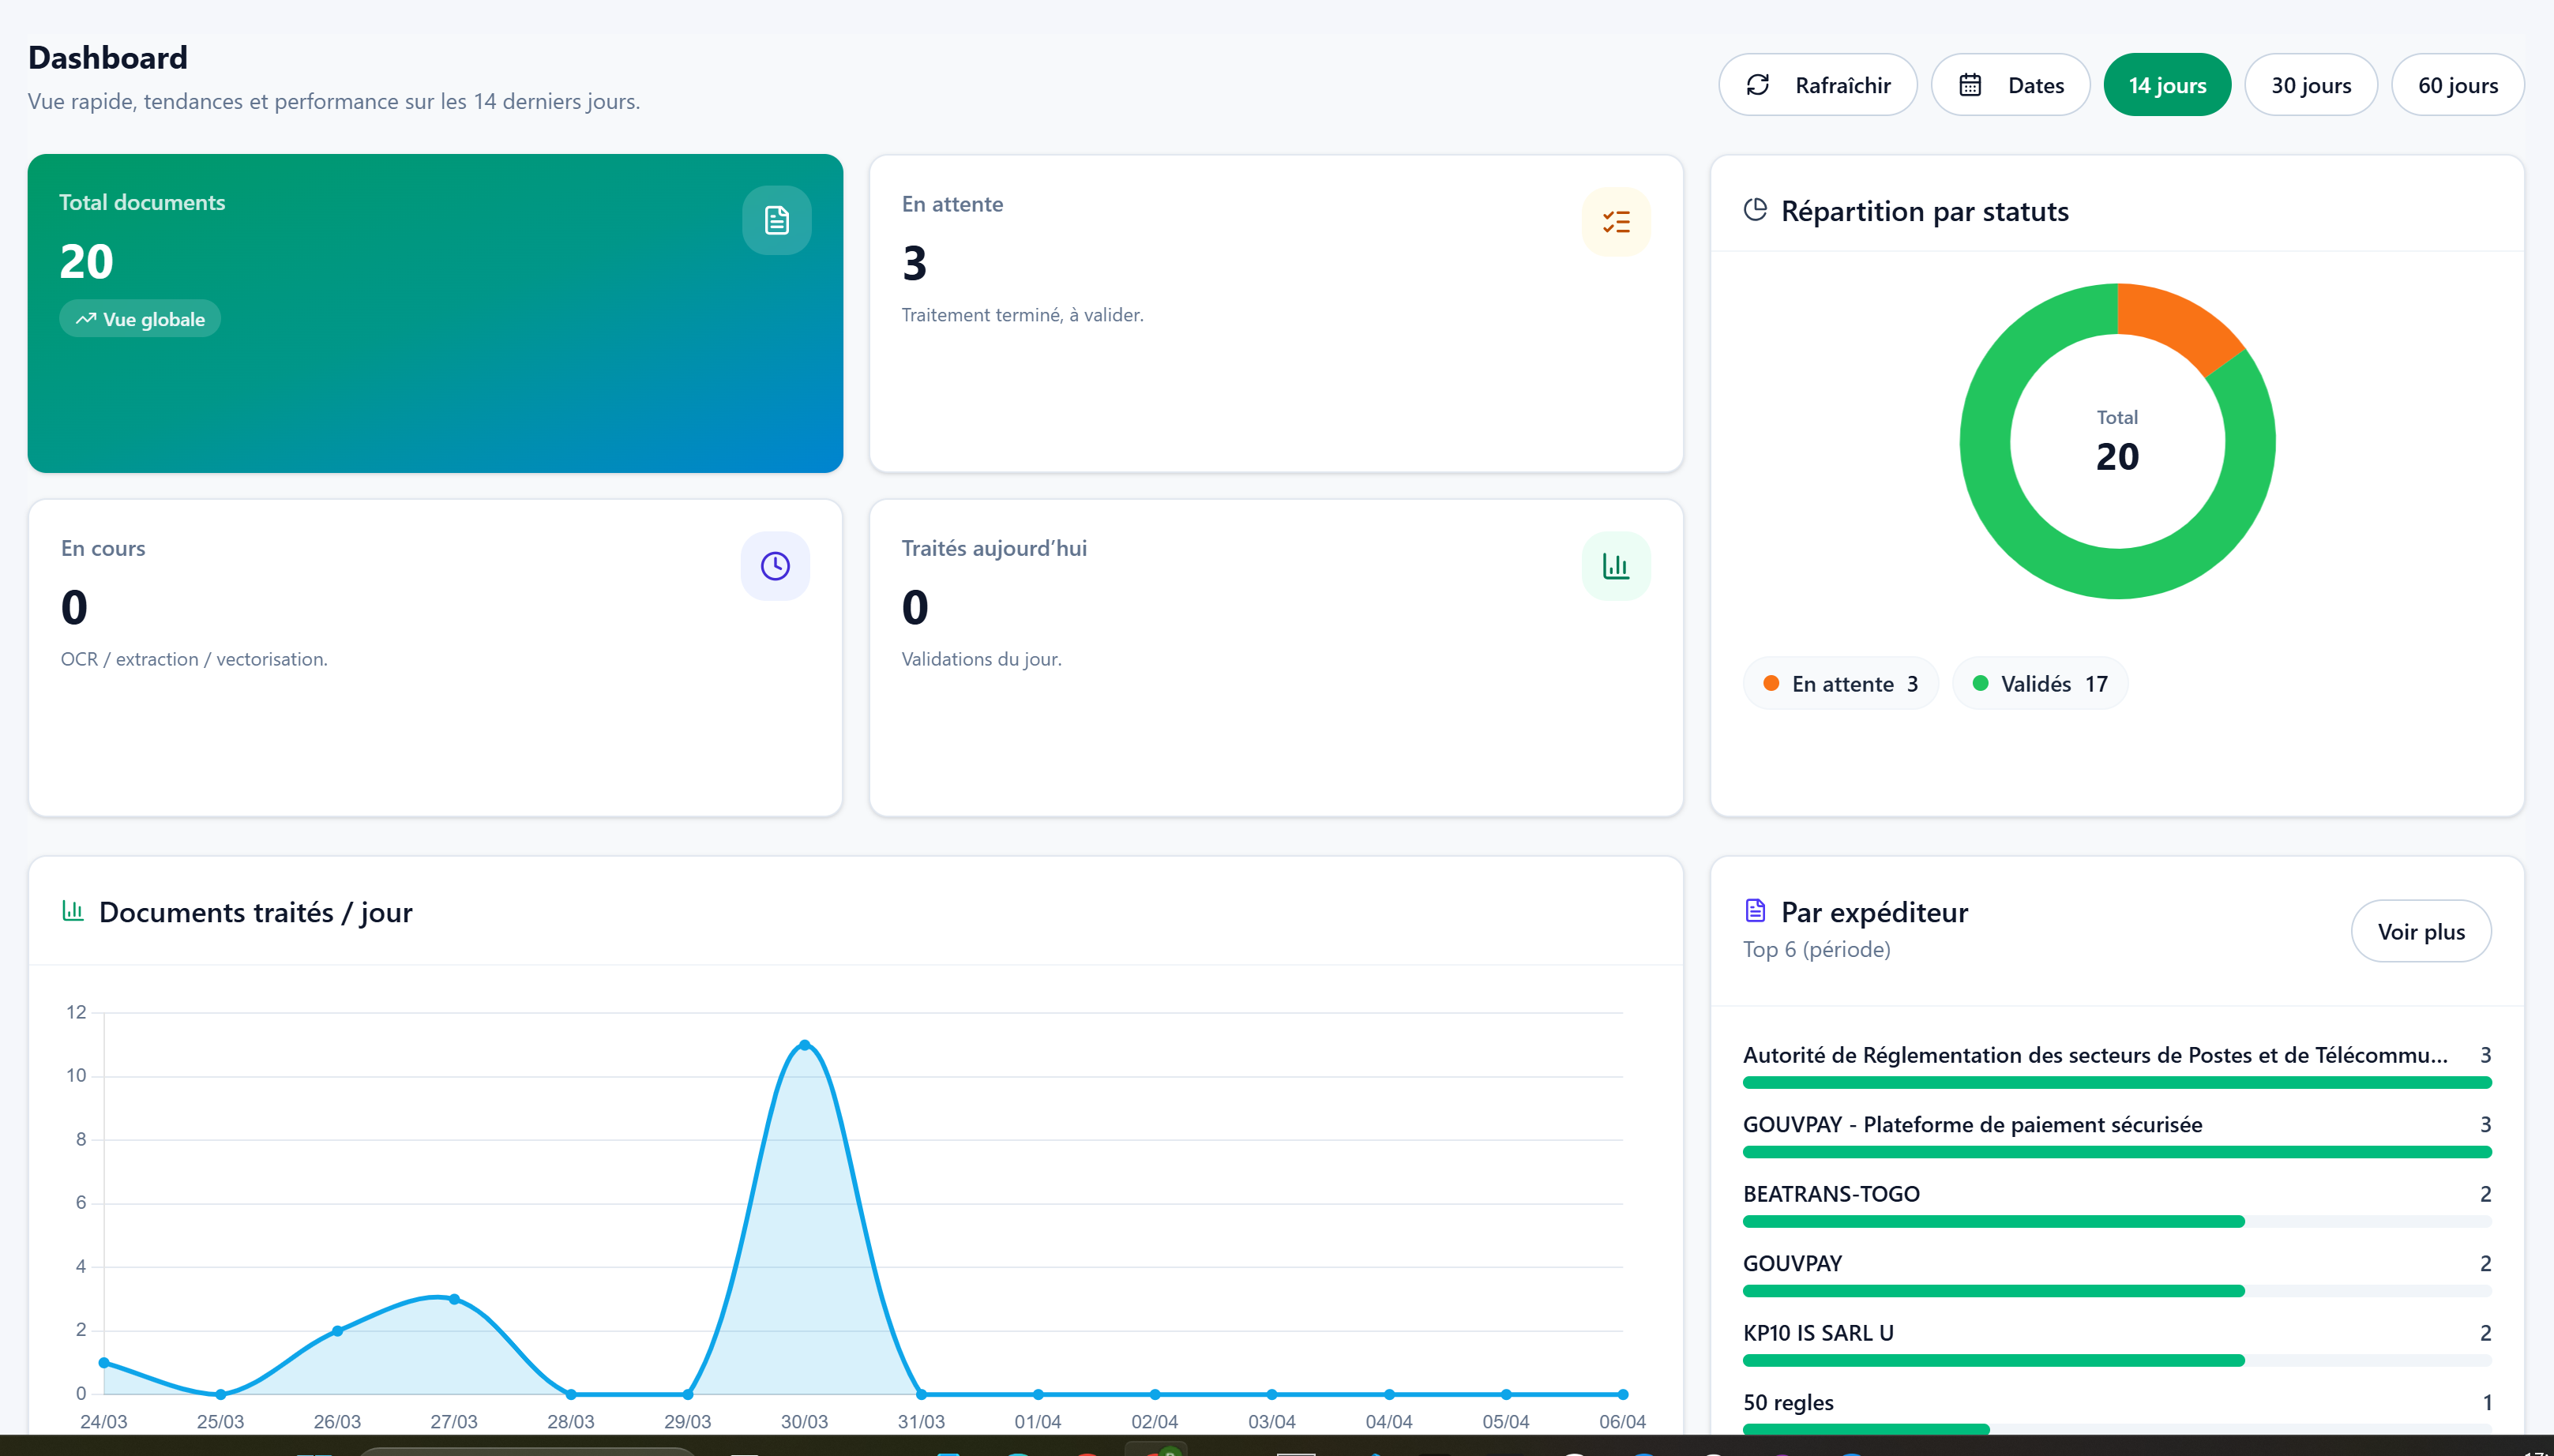
\includegraphics[width=0.98\textwidth]{images/screens/dashboard_1.png}
\par\vspace{0.6em}
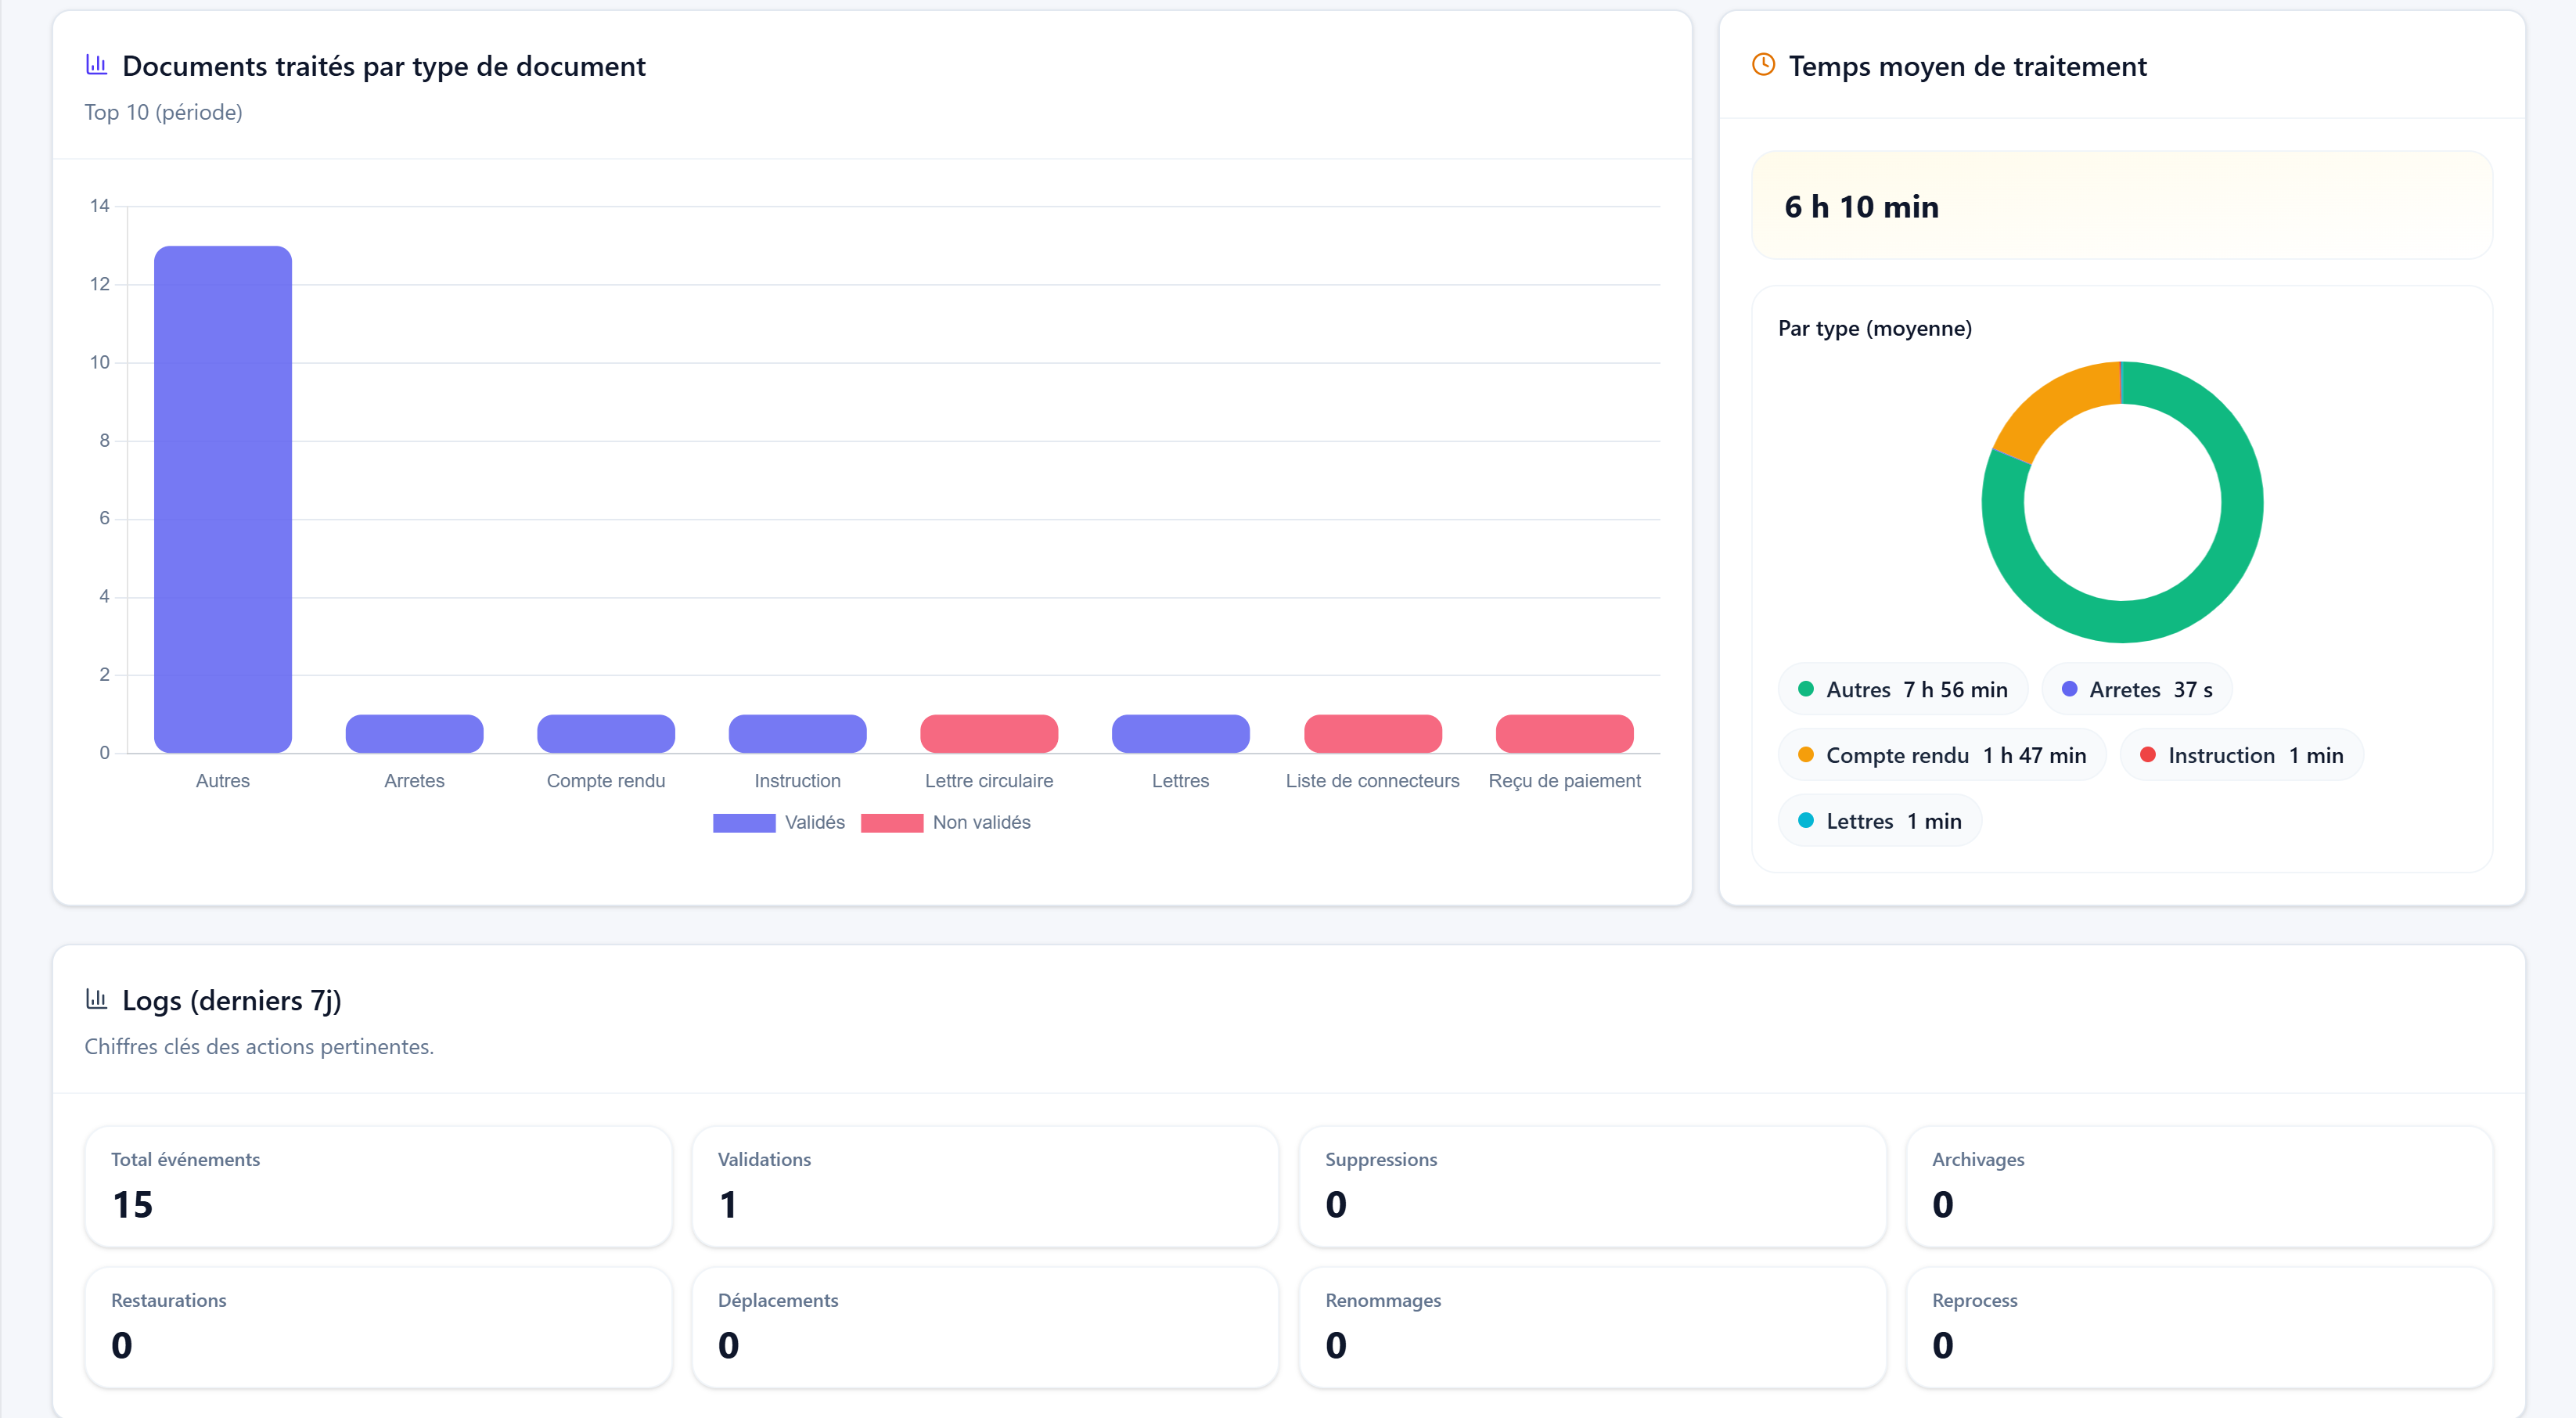
\includegraphics[width=0.98\textwidth]{images/screens/dashboard_2.png}
\caption{Tableaux de bord applicatifs : indicateurs de volumétrie, statuts, types de documents et temps moyen de traitement.}
\label{fig:dashboards-app}
\end{figure}

\section{Stack mise en place}
Une stack séparée est fournie :
\begin{itemize}
  \item \textbf{Prometheus} : collecte des métriques sur \texttt{/metrics} (FastAPI) et \texttt{/api/metrics} (Next.js) ;
  \item \textbf{Grafana} : dashboards et alerting, avec provisioning automatique ;
  \item \textbf{Loki} : stockage des logs ;
  \item \textbf{Vector} : collecte des logs Docker et expédition vers Loki.
\end{itemize}

\section{Alertes}
Des règles Prometheus détectent :
\begin{itemize}
  \item un taux d’erreurs HTTP 5xx supérieur à 5\% sur 10 minutes ;
  \item une latence p95 supérieure à 2s sur 10 minutes ;
  \item la présence d’erreurs OCR/extraction via des compteurs dédiés.
\end{itemize}

\chapter{Sécurité}
\section{Approche générale}
Le système est déployé \textbf{on-premise} afin de respecter les contraintes de souveraineté et de confidentialité propres à une administration publique. Dans ce contexte, l’architecture de sécurité s’inspire d’une approche \textbf{Zero Trust} : ne pas supposer qu’un réseau interne est sûr par défaut, limiter la surface exposée, vérifier systématiquement l’identité et appliquer des contrôles d’accès stricts.

\section{Exposition, réseau et segmentation}
L’exposition des composants est volontairement minimisée. Les accès externes sont concentrés sur un point d’entrée unique (reverse proxy), configuré en \textbf{TLS} afin de protéger les échanges. Les services internes (OCR, extraction, bus de messages, bases) restent non exposés et accessibles uniquement sur le réseau interne.

La segmentation réseau sépare les composants selon leur rôle (API/Frontend, traitements, stockage, observabilité, consoles). En production, les interfaces d’administration (RabbitMQ, MinIO, Grafana) sont restreintes (VPN, filtrage IP, comptes dédiés) afin d’éviter toute exposition accidentelle.

\section{Gestion des identités et des accès (IAM)}
La gestion des identités et des accès est un élément central pour sécuriser l’usage quotidien (secrétariats, administrateurs, services métier). Une intégration IAM est prévue via un fournisseur dédié (\textbf{Keycloak}) afin de :
\begin{itemize}
  \item centraliser l’authentification (\textbf{SSO}) et réduire la multiplication des comptes applicatifs ;
  \item gérer les rôles et groupes, et appliquer des politiques d’accès homogènes ;
  \item renforcer l’authentification (ex. \textbf{MFA}) selon la sensibilité des profils.
\end{itemize}
Cette approche facilite également la gestion du cycle de vie des comptes (création, révocation) et l’audit des connexions.

\section{Contrôle d’accès, RBAC et moindre privilège}
Le contrôle d’accès repose sur le principe du \textbf{moindre privilège} : chaque utilisateur et chaque service ne dispose que des droits strictement nécessaires. Le modèle RBAC (rôles et permissions) permet de limiter la consultation, la recherche et l’administration selon les profils, et de tracer les actions sensibles.

Au niveau des services, les permissions d’accès aux ressources (buckets MinIO, tables, files RabbitMQ) sont séparées et attribuées de manière fine, afin de réduire l’impact d’un éventuel compromis d’un composant.

\section{Gestion des secrets et configuration}
La configuration applicative est aujourd’hui centralisée via un fichier \texttt{.env} (développement). Pour une mise en production robuste, l’externalisation et la sécurisation des secrets est prévue avec \textbf{Vault} (HashiCorp Vault). L’objectif est d’éviter tout stockage en clair de mots de passe, clés API et tokens, et de permettre :
\begin{itemize}
  \item la rotation et la révocation des secrets ;
  \item la distribution contrôlée des secrets aux services autorisés ;
  \item la réduction du risque de fuite via les dépôts, logs ou sauvegardes.
\end{itemize}

\section{Traçabilité et journalisation}
La traçabilité est essentielle pour un environnement sensible : journalisation des actions (audit), suivi des traitements et corrélation des événements. Le système s’appuie sur :
\begin{itemize}
  \item un journal d’événements applicatifs (actions et changements d’état) ;
  \item des logs centralisés (Loki/Vector) et des métriques (Prometheus) pour détecter les anomalies ;
  \item des alertes (erreurs, latences, indisponibilités) afin de réduire le temps de réaction.
\end{itemize}
Ces mécanismes contribuent à la détection d’incidents, à l’analyse post-mortem et au respect des exigences d’audit.

\chapter{Évaluation du système RAG}
\section{Objectifs de l’évaluation}
L’intégration d’un mécanisme de recherche augmentée par génération (\textit{RAG}) vise à améliorer l’accès à l’information contenue dans les documents archivés. L’évaluation de ce système est essentielle afin de mesurer :
\begin{itemize}
  \item la pertinence des documents récupérés (\textit{retrieval}) ;
  \item la qualité des réponses générées (\textit{generation}) ;
  \item la cohérence entre les sources et les réponses fournies.
\end{itemize}

\section{Méthodologie envisagée}
L’évaluation du système RAG reposera sur la méthode \textbf{RAGAS} (\textit{Retrieval-Augmented Generation Assessment}), qui propose un cadre structuré pour mesurer les performances des systèmes RAG sans nécessiter de jeux de données annotés exhaustifs.

Les métriques envisagées incluent :
\begin{itemize}
  \item \textbf{Faithfulness} : cohérence entre la réponse générée et les documents sources ;
  \item \textbf{Answer Relevance} : pertinence de la réponse par rapport à la question ;
  \item \textbf{Context Precision} : qualité des documents récupérés ;
  \item \textbf{Context Recall} : capacité à récupérer les informations nécessaires.
\end{itemize}

\section{État d’avancement}
Les travaux d’évaluation sont actuellement en cours. Une première phase consiste à constituer un ensemble de requêtes représentatives des usages métier (recherche documentaire, consultation, assistance).

L’intégration de RAGAS permettra d’automatiser l’analyse des performances et d’identifier les axes d’amélioration, notamment :
\begin{itemize}
  \item la qualité des embeddings ;
  \item la stratégie de chunking ;
  \item le paramétrage des modèles de langage.
\end{itemize}

\section{Perspectives}
À terme, cette évaluation permettra :
\begin{itemize}
  \item d’optimiser la précision du système de recherche ;
  \item d’améliorer la fiabilité des réponses générées ;
  \item de garantir une meilleure adéquation aux besoins des utilisateurs métiers.
\end{itemize}

\chapter{Bilan de la mission et recommandations}
\section{Livrables et résultats}
Ce chapitre dresse un bilan global de la mission, en présentant les réalisations concrètes, les limites rencontrées, ainsi que les recommandations pour une mise en production et les enseignements tirés sur le plan personnel.

Au cours de la mission, une solution complète d’archivage numérique a été conçue et implémentée. Les principaux livrables incluent :
\begin{itemize}
  \item un pipeline de traitement automatisé couvrant l’ingestion des documents, l’OCR, l’extraction d’informations et l’indexation ;
  \item une architecture microservices assurant la modularité et la scalabilité du système ;
  \item une interface web permettant la consultation, la recherche et la validation des documents ;
  \item un système de recherche combinant recherche plein texte et recherche sémantique ;
  \item un assistant conversationnel basé sur une approche \textit{RAG} pour faciliter l’accès à l’information ;
  \item un déploiement en environnement \textit{on-premise} via Docker Compose ;
  \item une première couche d’observabilité incluant logs, métriques et tableaux de bord.
\end{itemize}

Les résultats observés sur un échantillon représentatif montrent :
\begin{itemize}
  \item une réduction significative des tâches manuelles liées au tri et au renommage ;
  \item une amélioration de la cohérence et de la qualité du classement documentaire ;
  \item une meilleure traçabilité des opérations grâce à la journalisation ;
  \item un accès plus rapide à l’information via la recherche et le chat documentaire.
\end{itemize}

\section{Limites et difficultés rencontrées}
Malgré les résultats obtenus, plusieurs limites et difficultés ont été identifiées.

\textbf{Sur le plan technique :}
\begin{itemize}
  \item la qualité variable des scans a un impact direct sur les performances de l’OCR ;
  \item l’hétérogénéité des formats documentaires complique l’extraction et la structuration des données ;
  \item certains traitements (OCR, extraction, embeddings) peuvent être coûteux en temps et en ressources.
\end{itemize}

\textbf{Sur le plan opérationnel :}
\begin{itemize}
  \item l’intégration dans un environnement contraint (réseau interne, sécurité) a nécessité des ajustements ;
  \item la gestion des volumes importants de documents impose une optimisation continue des performances ;
  \item la nécessité de conserver une validation humaine limite l’automatisation complète du processus.
\end{itemize}

Ces contraintes ont conduit à des arbitrages, notamment :
\begin{itemize}
  \item le choix d’un traitement asynchrone pour améliorer la robustesse ;
  \item la mise en place d’un workflow de validation utilisateur pour garantir la fiabilité ;
  \item une approche progressive privilégiant la qualité des résultats plutôt que l’automatisation totale.
\end{itemize}

\section{Bilan personnel}
Cette mission m’a permis de développer des compétences techniques et méthodologiques significatives dans la conception et la mise en œuvre de systèmes distribués orientés traitement documentaire.

\textbf{Sur le plan technique,} j’ai approfondi :
\begin{itemize}
  \item le développement d’architectures microservices (API, communication asynchrone) ;
  \item l’intégration de briques d’intelligence artificielle (OCR, extraction, \textit{RAG}) ;
  \item le déploiement et l’exploitation de solutions en environnement \textit{on-premise} (Docker, supervision).
\end{itemize}

\textbf{Sur le plan méthodologique,} cette expérience m’a permis de :
\begin{itemize}
  \item adopter une démarche itérative inspirée des méthodes agiles ;
  \item collaborer étroitement avec des utilisateurs métiers afin de mieux comprendre leurs besoins ;
  \item intégrer des contraintes réelles (performance, sécurité, exploitation) dans la conception.
\end{itemize}

Enfin, cette mission a également mis en évidence des axes d’amélioration, notamment :
\begin{itemize}
  \item approfondir les aspects liés à la sécurité des systèmes distribués ;
  \item améliorer l’optimisation des performances sur des volumes importants ;
  \item renforcer les pratiques de pilotage de projet et de formalisation des besoins.
\end{itemize}

\chapter*{Conclusion et perspectives}
\addcontentsline{toc}{chapter}{Conclusion et perspectives}
Le système développé constitue une chaîne d’archivage numérique complète, couvrant l’ensemble du cycle de vie du document, depuis la collecte automatique des scans jusqu’à leur consultation et leur recherche. En réduisant significativement les opérations manuelles (tri, renommage, saisie) et en proposant un classement plus homogène, la solution améliore à la fois la qualité de l’archivage et les délais de traitement.

Le choix d’un déploiement en environnement \textit{on-premise} permet de répondre aux exigences de sécurité et de souveraineté propres au contexte administratif, tandis que l’intégration de mécanismes d’observabilité contribue à une exploitation fiable et maîtrisée du système au quotidien. Par ailleurs, l’apport de techniques d’intelligence artificielle, notamment pour l’extraction d’informations et la recherche sémantique, renforce l’accessibilité et la valorisation du patrimoine documentaire.

Néanmoins, ce projet constitue une première étape vers un système d’archivage pleinement industrialisé. Plusieurs axes d’évolution peuvent être envisagés afin d’en améliorer la robustesse, la pertinence et l’intégration métier.

Les perspectives principales concernent :
\begin{itemize}
  \item l’amélioration des règles métier de classement, à travers la formalisation de référentiels documentaires, de modèles de nommage et la gestion des cas particuliers ;
  \item le renforcement des workflows de validation et de la gouvernance documentaire (gestion des droits, circuits de traitement, versioning) ;
  \item l’amélioration des capacités de recherche et d’assistance documentaire, notamment par l’optimisation des approches \textit{RAG} (qualité des contextes, citations, gestion des permissions) ;
  \item l’intégration de fonctionnalités complémentaires telles que la signature électronique, les politiques de conservation ou encore des tableaux de bord décisionnels.
\end{itemize}

À terme, l’évolution de ce système pourrait s’inscrire dans une démarche plus large de transformation numérique, visant à faire de la gestion documentaire un levier stratégique d’efficacité et de valorisation de l’information au sein de l’administration.

\chapter*{Références}
\addcontentsline{toc}{chapter}{Références}

\end{document}
